% siminos/presentations/APS20/APS20.tex        pdflatex APS18;; biber
% $Author: predrag $ $Date: 2020-03-01 15:09:21 -0500 (Sun, 01 Mar 2020) $

%  started with siminos/presentations/kittens/kittens.tex

                        \newif\ifboyscout\boyscouttrue          %% comments     %%
                        \newif\ifsubmission\submissionfalse     %% internal     %%
                        \newif\ifblog\blogfalse %% section shared with blogCats %%

\input ../../inputs/layoutBeamer
\usepackage[font=scriptsize, labelfont=bf]{caption}
\usepackage[
    backend=biber,  %bibtex,
    sorting=nyt,
    %refsection=chapter,
    %citereset=chapter,
    style=numeric, %alphabetic, % %style=authoryear,
    natbib=true,
    style=phys, % aps
    biblabel= brackets, % superscript, %
    articletitle=false, % true,  % false, % aps
    %chaptertitle=true,  % aip;  % false, % aps
    pageranges = true , % aip: the full range
             % = false, % aps: only the first page being printed
    sortlocale=en_US,
    firstinits=true,
    url=false, %true,  %
    doi=false, %true,
    eprint=false
]{biblatex}
\addbibresource{../../bibtex/siminos.bib}
\setbeamerfont{footnote}{size=\tiny}
%\input ../../inputs/def % no edits, always from dasbuch/book/inputs
\input ../kittens/defsKittens
\input ../../inputs/defsBeamer
\renewcommand{\Ssym}[1]{{\ensuremath{m_{#1}}}}    % Boris

\begin{document}

\title{
{\huge is space time?}
    \\
{a spatiotemporal tiling of turbulence}
}
\author{P. Cvitanovi\'c}
\author[Cvitanovi\'c]
{
  \textcolor{green!50!black}{
  {Predrag~Cvitanovi\'c, \\
  Han Liang
  and
  Matthew N Gudorf
  }	%\inst{1}
  }
}
\institute
{
%  \inst{1}%
\HREF{https://meetings.aps.org/Meeting/MAR20/Session/D37.2} {Session D37}:
    Transitional Flows \& Chaotic Dynamics:
    in honor of Bruno Eckhardt
\medskip

                (the canceled) APS March Meeting
 }
\date{March 2, 2020}

\begin{frame}
  \titlepage
\end{frame}

\begin{frame}{Bruno at Niels Bohr Institute, May 2006}
\begin{center}
\hfill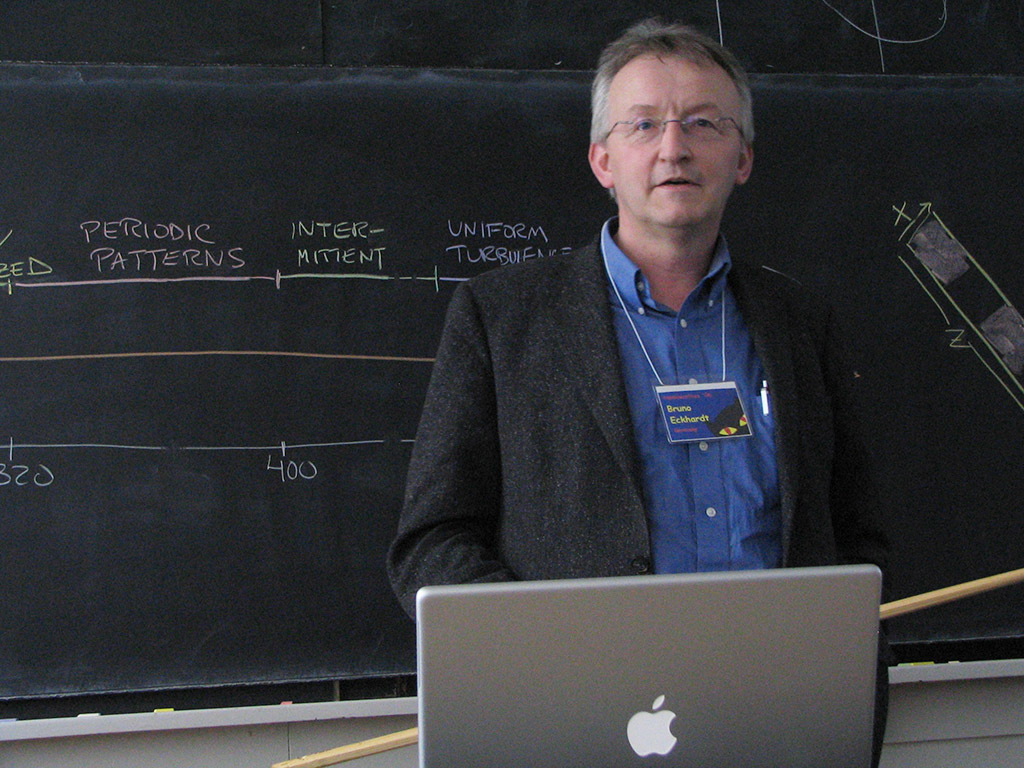
\includegraphics[width=1.00\textheight]{060519BrunoNBI}
\end{center}
\end{frame}

\begin{frame}{Bruno's secret}
\vfill

\begin{center}
{\Large keep it simple!}
\end{center}

\vfill
B Eckhardt\footfullcite{Eckhardt87}
{\em Fractal properties of scattering singularities}
(1987)
\bigskip

``$\cdots$ model studied is the motion of a particle in a plane,
elastically reflected by three circular discs centred on the corners of
an equilateral triangle''
\end{frame}

\begin{frame}{what is this? some background}
this talk is an introduction to the

\begin{center}
    {\textcolor{blue}{\catlatt}\footfullcite{CL18}}
\end{center}

the simplest example of the larger picture

\bigskip
\begin{center}
 \textcolor{blue}{spatiotemporal turbulence}\footfullcite{GuBuCv17}
\end{center}

\bigskip
that motivates our study of discrete \spt\ lattices
\end{frame}


\begin{frame}{motivation : need a theory of {\Huge large} fluid domains}
pipe flow close to onset of turbulence
\footnote{M.~Avila and B.~Hof, {Phys. Rev. \bf E 87} (2013)}
\begin{center}
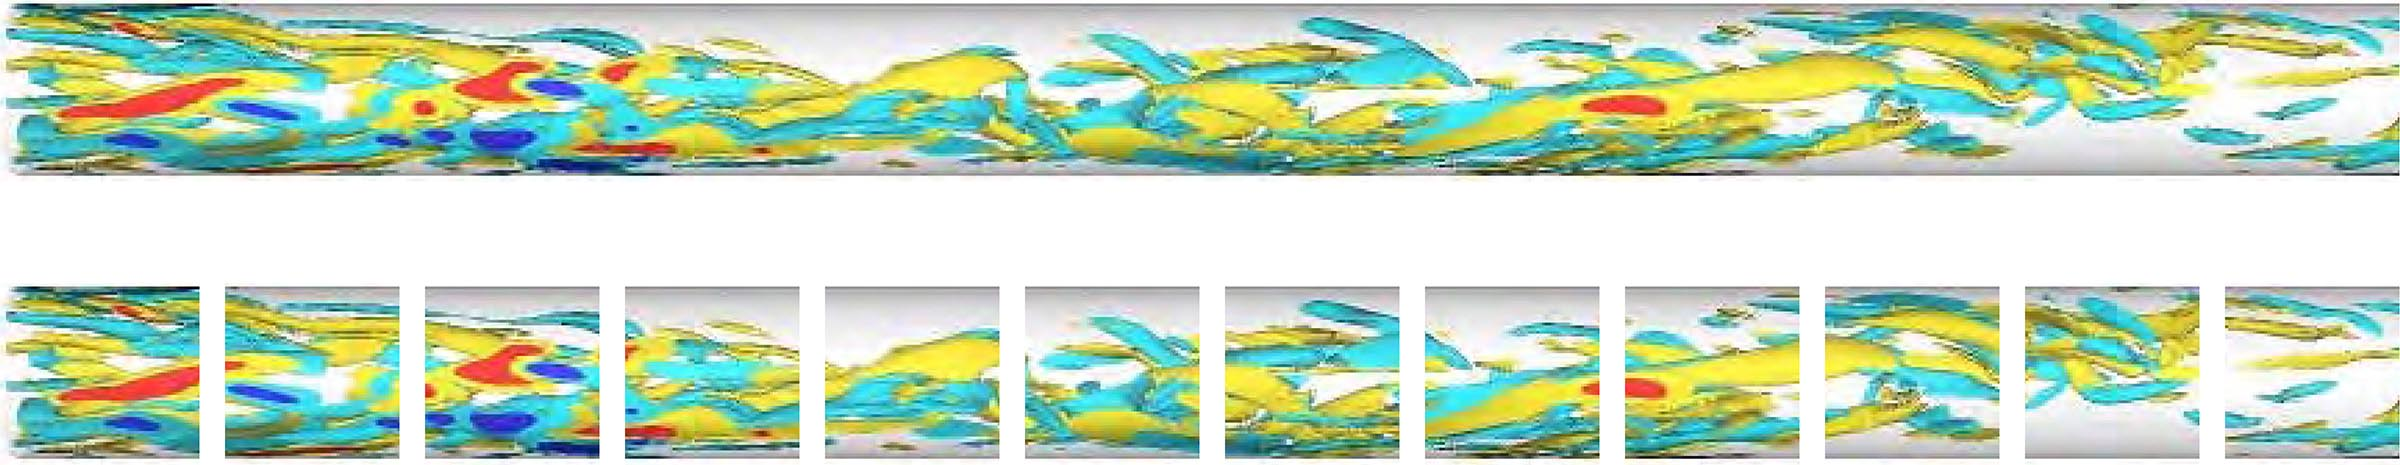
\includegraphics[width=1.0\textwidth]{AviHof13fig4CLM}
\end{center}
we have a detailed theory of {\small \textcolor{blue}{small}} turbulent fluid cells

\bigskip

can we construct the \textcolor{red}{infinite} pipe by coupling small turbulent cells ?
\bigskip

\textcolor{blue}{what would that theory look like ?}
\end{frame}


\begin{frame}{the goal}
\vfill

\begin{center}
{\Large build
\\
a chaotic field theory
\medskip

from
\\
the simplest chaotic blocks}
\end{center}

\vfill
using
\begin{itemize}
  \item
\textcolor{blue}{time invariance}
  \item
\textcolor{blue}{space invariance}
\end{itemize}
 of the defining partial differential equations
\end{frame}

\section[a coin toss]
 {a coin toss}

\begin{frame}{}
\begin{enumerate}
%              \item \textcolor{gray}{\small
%what this is about
%                  }
              \item {\Large
a coin toss
                  }\textcolor{gray}{\small
              \item
\templatt
              \item
\catlatt
              \item
bye bye, dynamics
                    }
            \end{enumerate}
\end{frame}

\renewcommand{\statesp}{state space}
\renewcommand{\ssp}{\ensuremath{x}}               % state space point

\begin{frame}{fair coin toss ~~~(AKA  {Bernoulli}  map)}
    \begin{block}{the essence of deterministic chaos}
\begin{center}
            \begin{minipage}[c]{0.36\textwidth}\begin{center}
% ChaosBook {fig:BernPartExam}
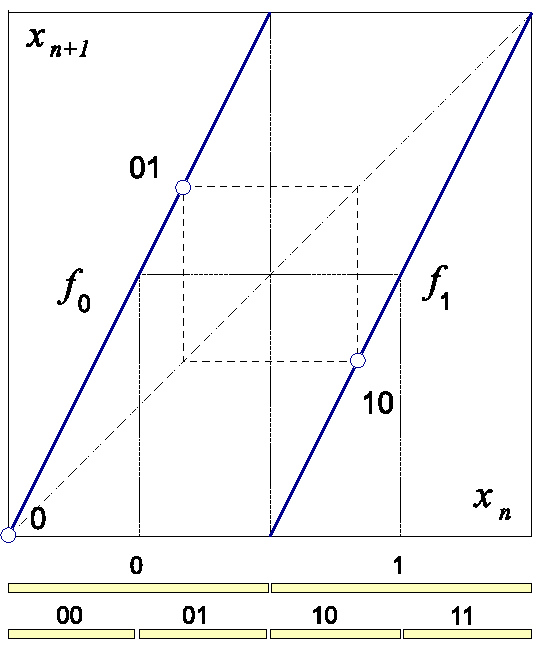
\includegraphics[width=1.0\textwidth]{BernPartCL18}
            \end{center}\end{minipage}
            \hspace{2ex}
            \begin{minipage}[c]{0.46\textwidth}\begin{center}
\[
\ssp_{\zeit+1} =
% \flow{}{\ssp_{\zeit}} =
\left\{ \begin{array}{l} %l}
        f_0(\ssp_{\zeit}) =  2 \ssp_{\zeit}
                             \\% \,, \quad & \ssp_{\zeit} \in \pS_0=[0,1/2) \\
        f_1(\ssp_{\zeit}) =  2 \ssp_{\zeit} \;\; (\mbox{mod}\;1)
                             % \,, \quad       & \ssp_{\zeit} \in \pS_1 =[1/2,1)
         \end{array}\right.
\]
            \end{center}\end{minipage}
\end{center}
%$\cl{}=2$ and 4 intervals \statesp\ partitions,

\hfill $\Rightarrow$~~~~~
fixed point \cycle{0}, 2-cycle \cycle{01}, $\cdots$
    \end{block}

\bigskip

a \HREF{https://www.random.org/coins/?num=2&cur=40-antique.aurelian}
{coin toss}

\hfill the simplest example of deterministic chaos
\end{frame}

\begin{frame}{what is ({mod}\;1) ?}
% linear
map with integer-valued `stretching' parameter $s\geq2$ :
\[
\ssp_{\zeit+1} \,=\, {s}\,\ssp_{\zeit}
\] %ee{BerStretch}

$(\mbox{mod}\;1)$ :
subtract the integer part
\(
\Ssym{\zeit+1}=\left\lfloor{s}\ssp_{\zeit}\right\rfloor
\)

\renewcommand{\ssp}{\ensuremath{\phi}}             % lattice site field
to keep fractional part
$\ssp_{\zeit+1}$ in the unit interval $[0,1)$
\[
\ssp_{\zeit+1}
= {s} \ssp_{\zeit} - \Ssym{\zeit+1}
\,,\qquad  \ssp_{\zeit}\in\pS_{\Ssym{\zeit}}
\] %ee{circ-m}
$\Ssym{\zeit}$ takes values in the ${s}$-letter alphabet
\[
\Ssym{\zeit} \in \A=\{0,1,2,\cdots,s-1\}
\] %ee{base-sAlph}
\end{frame}

\renewcommand{\ssp}{\ensuremath{\phi}}             % lattice site field
% \renewcommand{\Xx}{\ensuremath{\mathsf{\Phi}}}      % kittens lattice field
\begin{frame}{a fair dice throw}
    \begin{block}{slope ${6}$ Bernoulli map}
\begin{center}
            \begin{minipage}[c]{0.32\textwidth}\begin{center}
% ChaosBook {fig:BernPartExam}
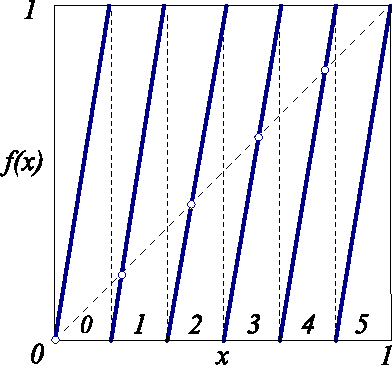
\includegraphics[width=1.0\textwidth]{fig_d_2CL18}
            \end{center}\end{minipage}
            \hspace{2ex}
            \begin{minipage}[c]{0.46\textwidth}
\(
\ssp_{\zeit+1}
= {6} \ssp_{\zeit} - \Ssym{\zeit+1}
\,,\;  \ssp_{\zeit}\in\pS_{\Ssym{\zeit}}
\)
\medskip

${6}$-letter alphabet \\
\(
\Ssym{\zeit} \in \A=\{0,1,2,\cdots,5\}
\)
            \end{minipage}
\end{center}
$6$ subintervals $\{\pS_{\Ssym{1}}\}$
    \end{block}
\end{frame}

\begin{frame}{what is chaos ?}
    \begin{block}{a fair dice throw}
\begin{center}
            \begin{minipage}[c]{0.32\textwidth}\begin{center}
% ChaosBook {fig:BernPartExam}
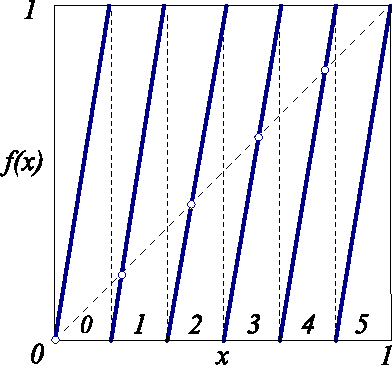
\includegraphics[width=1.0\textwidth]{fig_d_2CL18}
            \end{center}\end{minipage}
            \hspace{2ex}
            \begin{minipage}[c]{0.46\textwidth}
each subinterval contains a periodic point,
labeled by
$\Mm=\Ssym{1}\Ssym{2}\cdots\Ssym{\cl{}}$
\bigskip

$N_\cl{} = 6^\cl{}$ {\color{red}unstable} orbits
            \end{minipage}
\end{center}
$6$ subintervals $\{\pS_{\Ssym{1}}\}$,
$6^2$ subintervals $\{\pS_{\Ssym{1}\Ssym{2}}\}, \cdots$
    \end{block}
    \begin{block}{definition : chaos is}
positive Lyapunov $(\ln s)$ + positive entropy $(\frac{1}{\cl{}}\ln N_\cl{})$
    \end{block}
the precise sense in which

\hfill
\HREF{https://www.random.org/dice/}{dice throw}
is an example of deterministic chaos
\end{frame}

\renewcommand{\Xx}{\ensuremath{\Phi}}

\begin{frame}{lattice Bernoulli}
now recast the time-evolution Bernoulli map
\[
\ssp_{\zeit+1}
= {s} \ssp_{\zeit} - \Ssym{\zeit+1}
\] %ee{circ-m}
as a 1-step difference equation on the {\color{blue}temporal lattice}
\beq
\ssp_{\zeit} - {s}\ssp_{\zeit-1} = - \Ssym{\zeit}
\,,\qquad  \ssp_{\zeit} \in [0,1)
\ee{1stepDiffEq}
with a field $\ssp_\zeit$, source $\Ssym{\zeit}$ \\
on each site $\zeit$ of a
1\dmn\ lattice $\zeit\in\integers$
\bigskip

 write an \cl{}-sites lattice segment as \\
the {\color{blue}lattice state} and the {\color{blue}symbol \brick}
\beq
{\Xx} % = \{\ssp_j\}
             = (\ssp_{\zeit+1},\cdots,\ssp_{\zeit+\cl{}})
\,,\quad
{\Mm} % = \{\Ssym{j}\}
             = (\Ssym{{\zeit+1}},\cdots,\Ssym{{\zeit+\cl{}}})
\ee{pathBern}
\end{frame}

\begin{frame}{think globally, act locally}
Bernoulli equation at every instant $\zeit$, {\color{blue}local} in time
\beq
\ssp_{\zeit} - {s}\ssp_{\zeit-1} = - \Ssym{\zeit}
\ee{1stepDiffEq}
is enforced by the {\color{blue}global} equation
\beq
\left(\unit-{s}\hopMat^{-1}\right)\,\Xx = - \Mm
\,,
\ee{tempBern}
where the $[\cl{}\!\times\!\cl{}]$ matrix
\beq
\hopMat_{jk}=\delta_{j+1,k}
\,,\qquad
\hopMat
=  \left(\begin{array}{ccccc}
             0    &  1    &        &   &  \cr
                  &  0    &   1    &   &  \cr
                  &       &        & \ddots &  \cr
                  &       &        & 0 & 1 \cr
             1    &       &        &   & 0
          \end{array} \right)
\ee{hopMatrix}
implements the 1-time step operation
\end{frame}

\begin{frame}{think globally, act locally}
solving the {lattice Bernoulli} equation
\[
\jMorb\Xx= -\Mm
\,,
\]
with
the $[\cl{}\!\times\!\cl{}]$ matrix ~~~~~
\(
\jMorb = \unit-{s}{\hopMat}^{-1}
\,,
\) %{tempBernFix}
\medskip

can be viewed as a search for zeros of the function
\beq
F[\Xx] = \jMorb\Xx+\Mm = 0
\ee{tempFixPoint}
the entire {\color{blue}global lattice state} ${\Xx}_{\Mm}$ is now
\medskip

a single {\color{blue}fixed point}
$(\ssp_1,\ssp_{2},\cdots,\ssp_{\cl{}})$

\hfill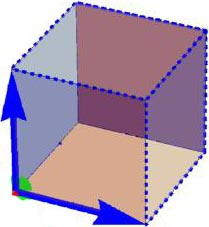
\includegraphics[width=0.12\textwidth]{hyperCube}

\hfill
in the \cl{}\dmn\ unit hyper-cube ~~~~~~~~~~~ $\Xx\in[0,1)^\cl{}$
\end{frame}

\begin{frame}{\jacobianOrb}
solving a nonlinear $F[\Xx]=0$ fixed point condition
with Newton method requires evaluation of
the $[\cl{}\!\times\!\cl{}]$ {\color{blue}\jacobianOrb}
\[
\jMorb_{ij} =\frac{\delta F[\Xx]_i}{\delta \ssp_j}
\] %ee{jacobianOrb}
what does this global \jacobianOrb\ do?
\bigskip

\begin{enumerate}
              \item
fundamental fact !
              \item
global stability of lattice state \Xx, perturbed everywhere
            \end{enumerate}
\end{frame}

\begin{frame}{(1) fundamental fact}
to satisfy the fixed point condition
\[
\jMorb\Xx+\Mm = 0
\]
the
 {\jacobianOrb} \jMorb\
\begin{enumerate}
              \item
stretches the unit hyper-cube $\Xx\in[0,1)^\cl{}$ into the \cl{}\dmn\
{\color{blue}\fundPip}
%\hfill\includegraphics[width=0.12\textwidth]{parallelepiped}
              \item
maps each periodic point ${\Xx}_{\Mm}$ into an integer lattice
$\integers^\cl{}$ point
              \item
then translate by integers $\Mm$ into the origin
            \end{enumerate}
hence $N_\cl{}$, the total number of solutions ~~=~~ the number of
{\color{blue}lattice points} within the {\fundPip}

\bigskip

the {\color{blue}fundamental fact}\footfullcite{BaHePl97} :
\[
N_\cl{} = |\Det\jMorb|
\] %ee{detBern0}
%\# integer points in {\fundPip} $=$ its volume
\end{frame}

\begin{frame}{example : {\fundPip} for $\cl{}=2$}
%$[2\!\times\!2]$

{\jacobianOrb}, unit
square basis vectors, their images :
\beq
\jMorb =
 \left(\begin{array}{cc}
  1 & -2 \\
 -2 &  1
 \end{array} \right)
;\quad
\Xx_B =
 \left(\begin{array}{c}
 1  \\
 0
 \end{array} \right)
\;\to\;
\Xx_{B'} = \jMorb\,\Xx_B =
 \left(\begin{array}{c}
  1  \\
 -2
 \end{array} \right)
\cdots\,,
\ee{bernFundPar}
%\medskip

    \begin{block}{Bernoulli periodic points of period 2}
\begin{center}
            \begin{minipage}[c]{0.32\textwidth}\begin{center}
% ChaosBook {fig:BernPartExam} % BernCyc2Jacob.svg
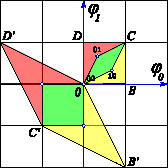
\includegraphics[width=1.0\textwidth]{BernCyc2JacobUnit}
            \end{center}\end{minipage}
            \hspace{2ex}
            \begin{minipage}[c]{0.46\textwidth}
$N_2=3$
\medskip


fixed point ~~$\Xx_{00}$\\
2-cycle ~~~~~~~$\Xx_{01}$, $\Xx_{10}$
            \end{minipage}
\end{center}
    \end{block}
\medskip

square $[0BCD]$
$\Rightarrow\jMorb\Rightarrow$
{\fundPip} $[0B'C'D']$
\end{frame}

\begin{frame}{fundamental fact is a fact for any $\cl{}$}

    \begin{block}{$\cl{}=3$ example} %{\templatt\ $\cl{}=3$ example}
$\jMorb\,$[unit hyper-cube] = [{\fundPip}]
\begin{center}
            \begin{minipage}[c]{0.32\textwidth}\begin{center}
% ChaosBook {fig:BernPartExam} % BernCyc2Jacob.svg
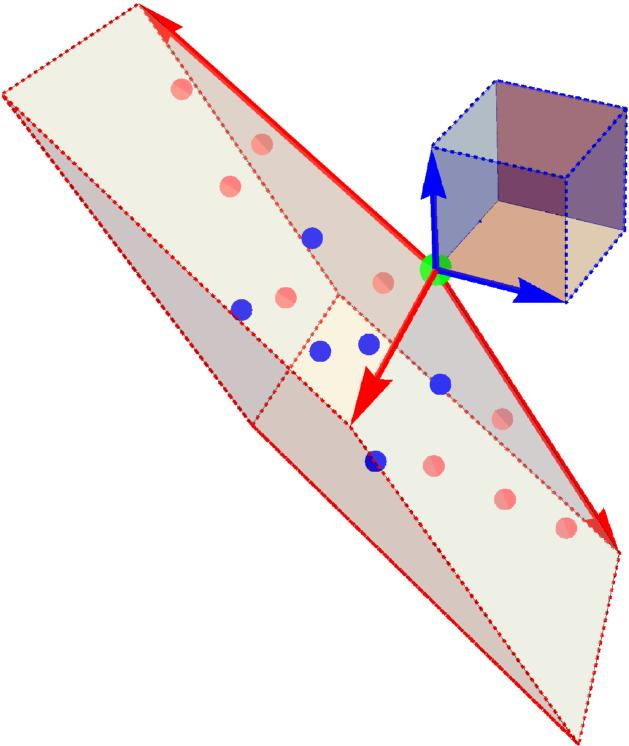
\includegraphics[width=1.0\textwidth]{PCLength3Counting}
            \end{center}\end{minipage}
            \hspace{2ex}
            \begin{minipage}[c]{0.46\textwidth}
unit hyper-cube $\Xx\in[0,1)^\cl{}$
\bigskip\bigskip

{\footnotesize $n>3$ cannot visualize}
            \end{minipage}
\end{center}
    \end{block}
    {\footnotesize
a periodic point $\rightarrow$ integer lattice point,
{\color{red}$\bullet$} on a face,
{\color{blue}$\bullet$} in the interior
    }
\end{frame}

\begin{frame}{(2) orbit stability vs. temporal stability}
\begin{block}{\jacobianOrb}
\(
\jMorb_{ij} =\frac{\delta F[\Xx]_i}{\delta \ssp_j}
\)
stability under {\color{blue}global} perturbation of the whole orbit

\hfill for \cl{} large, huge $[d\cl{}\!\times\!d\cl{}]$ matrix
\end{block}
\begin{block}{{\jacobianM}}
\(
\jMps^n
\)
propagates {\color{blue}initial} perturbation $\cl{}$ time steps

\hfill small $[d\!\times\!d]$ matrix
\end{block}
\vfill

$\jMps$ and $\jMorb$ are related by\footfullcite{Hill86}
\begin{block}{Hill's (1886) remarkable formula}
\[
|\Det\jMorb| = |\det(\matId - \jMps^n)|
%\label{catHillform}
\]
\end{block}
\end{frame}

\begin{frame}{by 1989 we forgot Bruno's secret}
\vfill

Cvitanovi\'c \& Eckhardt\footfullcite{CE89}
{\em Periodic orbit quantization of chaotic systems}
(1989)
\bigskip

``$\cdots$ computing from a few periodic orbits highly accurate estimates
of a large number of quantum resonances for the classically chaotic
3-disk scattering problem''

\vfill

\begin{center}
{\Large this time I'll keep it simple!}
\end{center}

\end{frame}

\begin{frame}{\po\ theory}
how come $\Det\jMorb$ counts periodic points ?
\bigskip

in 1984 Ozorio de Almeida and Hannay\footfullcite{OzoHan84} related the
number of periodic points to a \JacobianM\ by their
\begin{block}{principle of uniformity}
``periodic points of an ergodic system, counted with their natural
weighting, are uniformly dense in phase space''
\end{block}

where
\begin{block}{natural weight of \po\ {\Mm}}
\[
  \frac{1}{|\det(\unit - \jMps_{\Mm})|}
\]
\end{block}
\end{frame}

\begin{frame}{\po\ theory}
%how come a $\Det\jMorb$ counts  periodic points ?
\bigskip

``principle of uniformity'' is in\footfullcite{CBgetused}
\begin{block}{\po\ theory}
known as the \HREF{http://chaosbook.org/chapters/ChaosBook.pdf\#section.27.4} {flow
conservation} sum rule  :
\beq
\sum_{{\Mm}} %\ssp_i{\in\mbox{\footnotesize Fix}\map^{\cl{}}}}
    \frac{1}{|\det (\unit - \jMps_{\Mm})|}
    \;=
\sum_{{\Mm}} %{\ssp_i{\in\mbox{\footnotesize Fix}\map^{\cl{}}}}
    \frac{1}{|\Det\jMorb_{\Mm}|}
    =1
% \label{H-OdeA_mapsOrb}
\eeq
    {\footnotesize
sum over periodic points $\Xx_{\Mm}$ of period \cl{}
    }
\end{block}

\statesp\ is divided into

\hfill
{\color{blue}neighborhoods} of periodic points of period $\cl{}$
\end{frame}

\begin{frame}{\po\ theory}
how come a $\Det\jMorb$ counts periodic points ?
\bigskip

\begin{block}{flow conservation sum rule :}
\[
\sum_{\ssp_i{\in\mbox{\footnotesize Fix}\map^{\cl{}}}}
    \frac{1}{|\Det\jMorb_i|}
    =1
% \label{H-OdeA_mapsOrb}
\]
\end{block}
\medskip

%Bernoulli system `natural weighting' is simple :
%\medskip
%
%the determinant
%$\Det\jMorb_i=\Det\jMorb$ the same for all periodic points, whose
%number thus verifies the {\color{blue}fundamental fact}
%\[
%N_\cl{} = |\Det\jMorb|
%\] %ee{detBern0}

\vfill
    \begin{block}{the number of Bernoulli periodic lattice states}
\(
N_{\cl{}} = |\Det\jMorb| = s^{\cl{}} - 1
\) %\ee{noPerPtsBm}
~~~~~~~~for any $\cl{}$
    \end{block}
\end{frame}

\begin{frame}{\tzeta}
the {\color{blue}generating function} that sums up number of periodic
points $N_n$ to all orders is called {\color{blue}`topological zeta
function'}
\[
\zetatop(z)
 \,=\,  \exp \left(-\sum_{\cl{}=1}^\infty
\frac{z^\cl{}}{\cl{}} N_n
         \right)
\] %label{BernZeta}
for Bernoulli :
\[
\zetatop(z)
\,=\,
\frac{1 -  {s}z}{1 - z}
\]
%numerator $(1 - {s}z)$ says that Bernoulli orbits are built from \\
%$s$
%fundamental {\color{blue}primitive} lattice states,
%
%\hfill
%the fixed points
%$\{\ssp_0,\ssp_1,\cdots,\ssp_{s-1}\}$
%\medskip
%
%every other lattice state is
%built from their concatenations and repeats.

\vfill
\hfill {\Huge \textcolor{red}{solved!}}
\vfill

This is `\po\ theory'
\\
 And if you don't know,
\HREF{https://www.youtube.com/watch?v=_JZom_gVfuw} {now you know}

\end{frame}

\begin{frame}{coin toss ? that's not physics}
a field theory should be Hamiltonian, because
\bigskip

\begin{itemize}
  \item
that is physics
  \item
Quantum Mechanics demands it
\end{itemize}
\bigskip

need a system as simple
as the Bernoulli, but {\color{blue}mechanical}
\bigskip

so, we move on from running in circles,

\hfill
to a mechanical {\color{blue}rotor} to kick.
\end{frame}

\section[a kicked rotor]
 {a kicked rotor}

\begin{frame}{}
\begin{enumerate}
              \item \textcolor{gray}{\small
%what this is about
%              \item
a coin toss
                  }
              \item {\Large
a kicked rotor
                  }\textcolor{gray}{\small
              \item
\catlatt
              \item
bye bye, dynamics
                    }
            \end{enumerate}
\end{frame}


\begin{frame}{field theory in $1$ spacetime dimension}
we now define

\bigskip

\begin{block}{the cat map in $1$ spacetime dimension}
then we generalize to

\bigskip

$d$\dmn\ {\Large \catlatt}
\end{block}

\vfill

\begin{enumerate}
  \item cat map in Hamiltonian formulation
  \item cat map in Lagrangian formulation
    \hfill{\footnotesize (so much more elegant ! )}
\end{enumerate}
\end{frame}

\begin{frame}{(1) the traditional cat map}
\vfill

\begin{center}
{\huge Hamiltonian formulation}
\end{center}

\vfill
\end{frame}

\renewcommand{\statesp}{phase space}

\begin{frame}{example of a ``small domain'' dynamics : a single kicked rotor}
an electron circling an atom, subject to

a discrete time
sequence of angle-dependent kicks $F(x_{t})$

\hfill  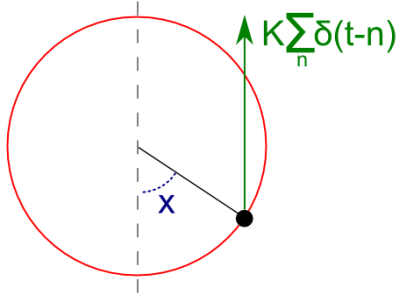
\includegraphics[width=0.33\textwidth]{kicked-rotor}

\begin{block}{Taylor, Chirikov and Greene  standard map}
\bea
x_{t+1} &=& x_{t}+p_{t+1} \qquad  \mod 1, \continue
p_{t+1} &=& p_{t} + F(x_{t})             \nnu
\eea
\end{block}

\medskip

\hfill $\to$ {\color{red}
chaos in Hamiltonian systems}
\end{frame}

\begin{frame}{the simplest example : a cat map evolving in time}

force
\(
 F(x) = Kx
\)
{\color{blue}linear} in the displacement $x$
\,,\;
$K\in\integers$
\bea
x_{t+1} &=& x_{t}+p_{t+1} \quad  \mod 1
        \continue
p_{t+1} &=& p_{t} + K x_{t} \qquad  \mod 1 \nnu
\eea
 \textcolor{red}{C}ontinuous
 \textcolor{red}{A}utomorphism of the
 \textcolor{red}{T}orus, or

\begin{block}{Hamiltonian cat map}
a linear, area preserving map of a 2-torus onto itself
 \[
 \left(\begin{array}{c}
   \ssp_{\zeit}  \\
   \ssp_{\zeit+1}
  \end{array} \right )=
  \jMps \left(\begin{array}{c}
   \ssp_{\zeit-1}  \\
   \ssp_{\zeit}
  \end{array} \right )
 - \left(\begin{array}{c}
 0  \\
 \Ssym{\zeit}
 \end{array} \right )
\,,\qquad
\jMps = \left (
\begin{array}{cc}
0 & 1 \\
-1 & s \\
\end{array}
    \right )
 \] %\ee{PerViv:2confRepMat}

\end{block}
for integer ``stretching''
$s=\tr{\jMps} > 2$ the map is \\ hyperbolic $\to$ a
fully chaotic Hamiltonian dynamical system
\end{frame}

\begin{frame}{(2) a modern cat}
\vfill
\begin{center}
{\huge Lagrangian formulation}
\end{center}
\vfill
\end{frame}

\begin{frame}{cat map in Lagrangian form}
replace momentum by velocity
\[
p_{t+1}=(\ssp_{t+1}  - \ssp_{t})/\Delta t
\]
formulation on temporal lattice
is pretty\footfullcite{PerViv} :
\begin{block}{2-step difference equation}
\[
\ssp_{t+1}  -  s \, \ssp_{t} + \ssp_{t-1}
    =
-\Ssym{t}
\] %\ee{eq:CatMapNewton1}
\end{block}
integer $\Ssym{t}$ ensures that

\hfill $\ssp_{t}$ lands in the unit interval

\bigskip
\[
\Ssym{t}\in  \A
\,,\quad \A\ = \{\mbox{finite alphabet}\}
\]
\end{frame}

\begin{frame}{think globally, act locally}
\templatt\ at every instant $\zeit$, {\color{blue}local} in time
\[
\ssp_{t+1}  -  s \, \ssp_{t} + \ssp_{t-1}
    =
-\Ssym{t}
\] %\ee{eq:CatMapNewton1}
is enforced by the {\color{blue}global} equation
\beq
(\hopMat - s\unit + \hopMat^{-1})\,\Xx = -\Mm
\,,
\ee{catTempLatt}
where
\end{frame}

\begin{frame}{\jacobianOrb}
\beq
{\Xx} % = \{\ssp_j\}
             = (\ssp_{\zeit+1},\cdots,\ssp_{\zeit+\cl{}})
\,,\quad
{\Mm} % = \{\Ssym{j}\}
             = (\Ssym{{\zeit+1}},\cdots,\Ssym{{\zeit+\cl{}}})
\ee{pathBern}
are a
{\color{blue}lattice state}, and a {\color{blue}symbol \brick}
\bigskip

and $[\cl{}\!\times\!\cl{}]$
 {\jacobianOrb} \jMorb\ is
\beq
\hopMat - s\unit + \hopMat^{-1}
=  \left(\begin{array}{ccccc}
            -s    &  1    &        &   & 1\cr
             1    & -s    &   1    &   &  \cr
                  &  1    &        & \ddots &  \cr
                  &       &        &-s & 1 \cr
             1    &       &        &   &-s
          \end{array} \right)
\ee{hopMatrix}
\end{frame}

\begin{frame}{think globally, act locally}
solving the \templatt\ equation
\[
\jMorb\Xx= -\Mm
\,,
\]
with
the $[\cl{}\!\times\!\cl{}]$ matrix ~~~~~
\(
\jMorb = \hopMat - s\unit + \hopMat^{-1}
\) %{tempBernFix}
\medskip

can be viewed as a search for zeros of the function
\beq
F[\Xx] = \jMorb\Xx+\Mm = 0
\ee{tempFixPoint}
where the entire {\color{blue}global lattice state} ${\Xx}_{\Mm}$ is
\medskip

a single {\color{blue}fixed point}
$(\ssp_1,\ssp_{2},\cdots,\ssp_{\cl{}})$

\hfill
in the \cl{}\dmn\ unit hyper-cube $\Xx\in[0,1)^\cl{}$
\end{frame}

\begin{frame}{fundamental fact in action}
% BernCyc2Jacob.svg
    \begin{block}{\templatt\  {\fundPip} for period 2}
square $[0BCD]$
$\Rightarrow\jMorb\Rightarrow$
{\fundPip} $[0B'C'D']$
\bigskip

\begin{center}
            \begin{minipage}[c]{0.32\textwidth}\begin{center}
% ChaosBook {fig:BernPartExam}
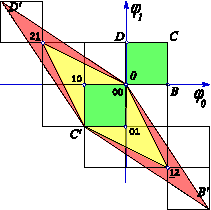
\includegraphics[width=1.0\textwidth]{catCyc2JacobUnit}
            \end{center}\end{minipage}
            \hspace{2ex}
            \begin{minipage}[c]{0.46\textwidth}
$N_2=|\Det\jMorb|=5$
\medskip

{\fundPip} \\
$=$  5 unit area quadrilaterals
            \end{minipage}
\end{center}
again, one periodic point per each unit volume
    \end{block}
\end{frame}

\begin{frame}{\templatt\ \tzeta}
again, can evaluate
\[
N_n=|\Det\jMorb|
\]
substitute the number of periodic points $N_n$ into the
{\color{blue}topological zeta func\-tion}
\bigskip

\bea
\zetatop(z)
 &=&  \exp \left(
    -\sum_{n=1} \frac{z^n}{n} N_n
    \right)
 \continue
 &=&  \frac{1 - s z + z^2}
                  {(1 - z)^2}
%\label{perOrbits:Isola90-13}
\eea

\vfill
{\Huge \textcolor{red}{solved!}}
\end{frame}

\begin{frame}{what continuum theory is \templatt\ discretization of?}
have
\begin{block}{2-step difference equation}
\[
\ssp_{t+1}  -  s \, \ssp_{t} + \ssp_{t-1}
    =
-\Ssym{t}
\] %\ee{eq:CatMapNewton1}
\end{block}
use discrete lattice derivatives
\begin{block}{Laplacian in $1$ dimension}
\[
\ssp_{t+1} - 2\ssp_{t} + \ssp_{t-1}
     =
\Box\,\ssp_t
\]
\end{block}
\medskip

to rewrite cat map as an (anti)oscillator chain
\begin{block}{$d=1$ damped Poisson equation (!)}
\[
 (\Box -s+2)\,\ssp_{t} = - \m_t
%    \,, \qquad
\] %\ee{LinearConn}
\end{block}
\vfill

\hfill
\textcolor{red}{did you know that a cat map can be so cool?}
\end{frame}

\begin{frame}{a reminder slide, to skip : Helmholtz equation in continuum}
\begin{block}{inhomogeneous Helmoltz equation}
is an elliptical equation of form
\beq
   (\Box+k^2)\,\ssp(x)= -\Ssym{}(x)\,,\qquad x\in \reals^d
\label{CatMapContinuesPC}
\eeq
where $\ssp(x)$ is a $C^2$ function, and $\Ssym{}(x)$ is a function
with compact support
\end{block}

\bigskip

for the $\lambda^2=-k^2>0$ (imaginary $k$), the equation is known as  the
{\color{blue}screened Poisson equation}\footfullcite{FetWal03}, or the Yukawa
equation
\end{frame}

\begin{frame}{that's it! for spacetime of $1$ dimension}
lattice damped Poisson equation
    {\Huge
\[
 (\Box -s+2)\ssp_{z} = - \m_z
%    \,, \qquad
\] %\ee{LinearConn}
    }
\hfill solved completely and analytically!
\end{frame}

\begin{frame}{think globally, act locally - summary}
\bigskip
the problem of enumerating and determining all global solutions stripped
to its essentials :
\bigskip
\begin{enumerate}
              \item
each solution is a zero of the global fixed point condition
\[
F[\Xx] = 0
\]
              \item
global stability :  the {\jacobianOrb}
\[
\jMorb_{ij} =\frac{\delta F[\Xx]_i}{\delta \ssp_j}
\]
              \item
{\color{blue}fundamental fact} : the number of period-$\cl{}$ orbits
\[
N_\cl{} = |\Det\jMorb|
\]

              \item
zeta function $\zetatop(z)$ : all predictions of the theory
            \end{enumerate}
\end{frame}

\section[\catlatt]
 {\catlatt}
\label{s:catLatt}

\begin{frame}{}
\begin{enumerate}
              \item \textcolor{gray}{\small
%what this is about
%              \item
a coin toss
              \item
a kicked rotor
                  }
              \item {\Large
\catlatt
                  }\textcolor{gray}{\small
              \item
bye bye, dynamics
                    }
            \end{enumerate}
\end{frame}

\begin{frame}{herding cats in $d$ spacetime dimensions}
start with
\begin{block}{a cat map at each lattice site}
\bigskip

talk to neighbors
\medskip

spacetime $d$\dmn\
~~~~~~~ {\color{blue}\Large \catlatt}
\end{block}

\vfill

\begin{itemize}
  \item Hamiltonian formulation \hfill{\footnotesize (awkward, forget about it)}
  \item Lagrangian formulation \hfill{\footnotesize (elegant)}
\end{itemize}
\end{frame}

\begin{frame}{\catlatt}
consider
a 1 spatial dimension lattice, with field
$\ssp_{nt}$ \\
(the angle of a kicked
rotor ``particle'' at instant $t$, at site $n$)
\begin{block}{require}
\begin{itemize}
\item  each site couples to
its nearest neighbors $\ssp_{n\pm1,t}$
\item  invariance under
spatial translations
\item  invariance under spatial reflections
\item  invariance under the space-time exchange
\end{itemize}
\end{block}

\bigskip

obtain\footfullcite{GutOsi15}
\begin{block}{2\dmn\ coupled cat map lattice}
\[
\ssp_{n,t+1} + \ssp_{n,t-1} - 2s \, \ssp_{n t} + \ssp_{n+1,t} + \ssp_{n-1, t}
     =-\Ssym{n t}
\] %\ee{eq:CatMapNewton2}
\end{block}
\end{frame}

\begin{frame}{herding cats : a discrete Euclidean space-time field theory}
write the spatial-temporal differences as discrete derivatives
\begin{block}{Laplacian : in $d=1$ and $d=2$ dimensions}
\(
\Box\,\ssp_t \;\;\,=\, \ssp_{t+1} - 2\ssp_{t} + \ssp_{t-1}
\)\\ \(
\Box\,\ssp_{nt} \,=\, \ssp_{n,t+1} + \ssp_{n,t-1}
- 4 \, \ssp_{nt} + \ssp_{n+1,t} + \ssp_{n-1, t}
\)
\end{block}
\(
-\Ssym{n t}
 =
\ssp_{n,t+1} + \ssp_{n,t-1} - 2s \, \ssp_{n t} + \ssp_{n+1,t} + \ssp_{n-1, t}
\) %\ee{eq:CatMapNewton2}

\bigskip

the cat map is thus generalized  to
\begin{block}{$d$\dmn\ \catlatt}
\[
 (\Box - d(s-2))\ssp_{z} = - \m_z
%    \,, \qquad
\] %\ee{LinearConn}

\medskip

\end{block}

\bigskip

where
\(
  \ssp_{z} \in  \mathbb{T}^{1}
    \,, \quad
  \Ssym{z} \in \A
    \mbox{  and  }
  z\in \integers^{d}
\) = lattice sites
\end{frame}

\begin{frame}{spatiotemporally infinite `\catlatt'}
%\begin{center}
%\hfill
\includegraphics[width=0.55\textwidth]{spatiotempCat}
\hfill
\includegraphics[width=0.55\textwidth]{DawnBishopCats}
%\end{center}
\end{frame}

\begin{frame}{discretized linear PDE}
\begin{block}{$d$\dmn\ \catlatt}
{\Large
\[
 (\Box -d(s-2))\,\ssp_{z} = - \Ssym{}_z
%    \,, \qquad
\] %\ee{LinearConn}
}
\end{block}

\bigskip

is linear and known as
\begin{itemize}
\item {\color{blue}Helmholtz} equation if stretching is weak, $s<2$ \\
(oscillatory sine, cosine solutions)
\item damped {\color{blue}Poisson} equation if stretching is strong, $s>2$ \\
(hyperbolic sinches, coshes)
\end{itemize}
the nonlinearity is hidden in the ``source''
\[
  \Ssym{z} \in \A
    \mbox{  at lattice site  }
  z\in \integers^{d}
\]
\end{frame}

\begin{frame}{the simplest of all `turbulent' field theories ! }
\catlatt
\[
 (\Box -d(s-2))\ssp_{z} = - \m_z
%    \,, \qquad
\] %\ee{LinearConn}
\bigskip
\hfill can be solved completely (?) and analytically (!)

\bigskip
\bigskip

assign to each site $z$ a
letter \Ssym{z}\ from the alphabet $\A$.

\medskip

a particular fixed set
of letters  \Ssym{z}\ (a lattice state)
\[
\Mm= \{\Ssym{z}\} % \in \A \,,\; z\in \integers^d \}
 = \{\Ssym{n_1 n_2 \cdots n_d}\}
\,,
\]
is a complete specification of the corresponding \\
lattice state $\Xx$
\bigskip

{\color{blue}\footnotesize
(from now on work in $d=2$ dimensions, `stretching parameter' $s=5/2$)
}
\end{frame}

\begin{frame}{think globally, act locally}
solving the \catlatt\ equation
\[
\jMorb\Xx= -\Mm
\,,
\]
with
the $[\cl{}\!\times\!\cl{}]$ matrix ~~~~~
\(
\jMorb = \sum_{j=1}^{2}\left(\hopMat_j-{s}\unit+\hopMat_{j}^{-1}\right)
\) %{tempBernFix}
\medskip

can be viewed as a search for zeros of the function
\beq
F[\Xx] = \jMorb\Xx+\Mm = 0
\ee{tempFixPoint}
where the entire {\color{blue}global lattice state} ${\Xx}_{\Mm}$ is
\medskip

a single {\color{blue}fixed point}
${\Xx}_{\Mm}=\{\ssp_z\}$

\hfill
in the \speriod{}\period{}\dmn\ unit hyper-cube $\Xx\in[0,1)^{\speriod{}\period{}}$
\medskip

$\speriod{}$ is the `spatial',
$\period{}$ the `temporal' lattice period
\end{frame}

\begin{frame}{Bravais lattices}
2\dmn\ \emph{Bravais lattice} is an infinite array of points
\beq
\Lambda = \{n_1 {\bf a}_1 + n_2 {\bf a}_2\,|\,n_i \in \mathbb{Z}\}
\ee{2DBravaisLattice}
    \begin{block}{example : $[3\!\times\!2]_1$ Bravais tile}
\begin{center}
            \begin{minipage}[c]{0.32\textwidth}\begin{center}
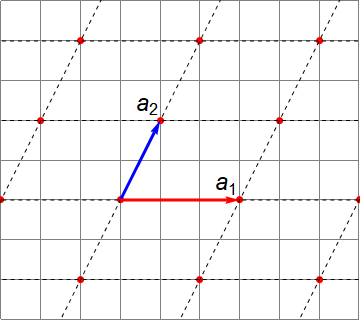
\includegraphics[width=1.0\textwidth]{HLBravaisLattice}
            \end{center}\end{minipage}
            \hspace{2ex}
            \begin{minipage}[c]{0.46\textwidth}
basis vectors \\ ${\bf a}_1=(3,0)$, ${\bf a}_2=(1,2)$
            \end{minipage}
\end{center}
    \end{block}

\vfill

6 field values, on 6 lattice sites $z=(n,\zeit)$,
$[3\!\times\!2]$ rectangle:
\[
 \left[
 \begin{array}{ccc}
 \ssp_{01} & \ssp_{11} & \ssp_{21} \\
 \ssp_{00} & \ssp_{10} & \ssp_{20}
 \end{array}
 \right]
\]
\end{frame}

\begin{frame}{fundamental fact works in spacetime (!)}

    \begin{block}{recall Bernoulli example ?}
\begin{center}
            \begin{minipage}[c]{0.32\textwidth}\begin{center}
% ChaosBook {fig:BernPartExam} % BernCyc2Jacob.svg
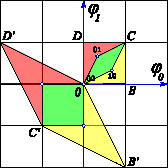
\includegraphics[width=1.0\textwidth]{BernCyc2JacobUnit}
            \end{center}\end{minipage}
            \hspace{2ex}
            \begin{minipage}[c]{0.46\textwidth}
$[0BCD]$ : \\
unit hyper-cube $\Xx\in[0,1)^\cl{}$
\medskip

$[0B'C'D']$ : \\
{\fundPip}
            \end{minipage}
\end{center}
$\jMorb\,[0BCD] =$ {\fundPip} $[0B'C'D']$
    \end{block}

\vfill

any spacetime, {\fundPip} basis
vectors $\jEigvec[j]$ \\
$=$ columns of the {\jacobianOrb}
\beq
\jMorb = (\jEigvec[1]|\jEigvec[2]|\cdots|\jEigvec[\cl{}])
\ee{lattJac}
\end{frame}


%\begin{frame}{solving $1D$ cat map using Green's functions}
%\begin{block}{the Green's function $\Xx=g\,\Mm$ for a period \period{} solution of}
%\[
% (\Box -s+2)\ssp_{t} = \m_t
%%    \,, \qquad
%\] %\ee{LinearConn}
%
%\medskip
%\end{block}
%\begin{block}{is a Toeplitz matrix $\gd$ that satisfies}
%\bea
% (\D \gd)_{tt'}&=&\delta_{tt'}\,, \qquad t,t'\in 0,1,2,\cdots,\period{}-1
%% \label{1DGreenFun0} \ee{1DGreenFunDirichlet}
%        \continue
%   & &  \continue
%\D &=&\left(\begin{array}{ccccccc}
% s&-1 & 0 & 0 &\dots &0&-1 \\
%-1 &  s&-1 & 0 &\dots &0&0 \\
%0 &-1 &  s&-1 &\dots &0 & 0 \\
%\vdots & \vdots &\vdots & \vdots & \ddots &\vdots &\vdots\\
%0 & 0 & \dots &\dots &\dots  & s&-1 \\
%-1 & 0 & \dots &  \dots &\dots&-1 &  s
%        \end{array} \right )
%\nnu
%\eea %ee{3diagToeplitz}
%\medskip
%\end{block}
%\end{frame}

%\begin{frame}{
%the 3-letter translations alphabet \;+\; the Markov graph
%             }
%
%\medskip
%
%generates the admissible orbits of $1D$ cat map
%\[ %beq
%\Ssym{t}\in\{\underline{1},0,1\}
%\] %ee{threeLett}
%example : all admissible 4-cycles
%\bea
%{\bf x}_{0 0 1 \underline{1}} &=& \frac{1}{15}
%\left[
%\begin{array}{cccc}
% {-1} &
% {1} &
% {4} &
% {-4}
%\end{array}
%\right]
%    \,,\qquad
%{\bf x}_{0 1 0 \underline{1}}= \frac{1}{15}
%\left[
%\begin{array}{cccc}
% {0} &
% {5} &
% {0} &
% {-5}
%\end{array}
%\right]
%    \continue
%{\bf x}_{0 1 \underline{1}1} &=& \frac{1}{15}
%\left[
%\begin{array}{cccc}
% {4} &
% {6} &
% {-1} &
% {6}
%\end{array}
%\right]
%    \,,\qquad
%{\bf x}_{0 1 1 \underline{1}}= \frac{1}{15}
%\left[
%\begin{array}{cccc}
% {2} &
% {8} &
% {7} &
% {-2}
%\end{array}
%\right]
%    \continue
%% Predrag 2018-02-19 replaced the
%% old 6 \cycle{3125} \\  1 0 1 \underline{1} = 4 \cycle{1253}
%% by new No. 6:
%% 6 \cycle{1133} \\  0 0 1            1
%{\bf x}_{0 0 1 1} &=& \frac{1}{15}
%\left[
%\begin{array}{cccc}
% {5} &
% {5} &
% {10} &
% {10}
%\end{array}
%\right]
%    \,,\qquad
%{\bf x}_{1 1 1 \underline{1}}= \frac{1}{15}
%\left[
%\begin{array}{cccc}
% {9} &
% {11} &
% {9} &
% {1}
%\end{array}
%\right]
%    \continue
%{\bf x}_{1 1 1 0} &=& \frac{1}{15}
%\left[
%\begin{array}{cccc}
% {12} &
% {13} &
% {12} &
% {8}
%\end{array}
%\right]
%    \,,\qquad
%{\bf x}_{1 1 0 \underline{1}}= \frac{1}{15}
%\left[
%\begin{array}{cccc}
% {7} &
% {8} &
% {2} &
% {-2}
%\end{array}
%\right]
%    \continue
%{\bf x}_{0 0 \underline{1}1} &=& \frac{1}{15}
%\left[
%\begin{array}{cccc}
% {1} &
% {-1} &
% {-4} &
% {4}
%\end{array}
%\right]
%\label{4cyclesPerPoints}
%\eea
%\end{frame}

\begin{frame}{example : spacetime periodic $[3\!\times\!2]$ Bravais \brick}
\[
F[\Xx] = \jMorb\Xx+\Mm = 0
\]
6 field values, on 6 lattice sites $z=(n,\zeit)$,
$[3\!\times\!2]$ rectangle:
\[
 \left[
 \begin{array}{ccc}
 \ssp_{01} & \ssp_{11} & \ssp_{21} \\
 \ssp_{00} & \ssp_{10} & \ssp_{20}
 \end{array}
 \right]
\]
\[
z=(\ell t),z'=(\ell' t')\in T^2_{[3\!\times\!2]}
\]

\medskip

vectors and matrices can be written in block form, vectors as 1\dmn\ arrays,
\beq
\Xx_{[3\!\times\!2]} =
\left(\begin{array}{c}
 \ssp_{01} \\
 \ssp_{00} \\
  \hline
 \ssp_{11} \\
 \ssp_{10} \\
  \hline
 \ssp_{21} \\
 \ssp_{20} \\
      \end{array}\right)
\,,\qquad
\Mm_{[3\!\times\!2]} =
\left(\begin{array}{c}
 \Ssym{01} \\
 \Ssym{00} \\
  \hline
 \Ssym{11} \\
 \Ssym{10} \\
  \hline
 \Ssym{21} \\
 \Ssym{20} \\
        \end{array}\right)
\ee{3times2blockVect}
\end{frame}

\begin{frame}{}
with the $[6\!\times\!6]$ {\jacobianOrb} in block-matrix form
\beq
\jMorb_{[3\!\times\!2]} =
\left(
\begin{array}{cc|cc|cc}
 -2 s & 2 & 1 & 0 & 1 & 0  \\
 2 & -2 s & 0 & 1 & 0 & 1  \\
  \hline
 1 & 0 & -2 s & 2 & 1 & 0  \\
 0 & 1 & 2 & -2 s & 0 & 1  \\
  \hline
 1 & 0 & 1 & 0 & -2 s & 2  \\
 0 & 1 & 0 & 1 & 2 & -2 s
\end{array}
\right)
\ee{3times2basisVecs}
\end{frame}

\begin{frame}{}

{\fundPip} basis
vectors $\jEigvec[j]$ are
the columns of the {\jacobianOrb}
\beq
\jMorb_{[3\!\times\!2]} =
\left(
\begin{array}{c|c|c|c|c|c}
 -2 s & 2 & 1 & 0 & 1 & 0  \\
 2 & -2 s & 0 & 1 & 0 & 1  \\
 1 & 0 & -2 s & 2 & 1 & 0  \\
 0 & 1 & 2 & -2 s & 0 & 1  \\
 1 & 0 & 1 & 0 & -2 s & 2  \\
 0 & 1 & 0 & 1 & 2 & -2 s
\end{array}
\right)
\ee{3times2basisVecs}
the `fundamental fact' now yields the number of
solutions for any ${s}$
\beq
N_{[3\!\times\!2]} = |\Det\jMorb_{[3\!\times\!2]}|
                   = 4({s}-2)s(2{s}-1)^2 (2{s}+3)^2
\ee{N3times2}
\end{frame}

\begin{frame}{counting \catlatt\ solutions}

\begin{enumerate}
  \item can construct Bravais spacetime tilings,
  from small tiles to as large as you wish
  \item for each Bravais spacetime tile $[\speriod{}\!\times\!\period{}]_S$,
can evaluate
\[
N_{[\speriod{}\!\times\!\period{}]_S}
\]
\end{enumerate}
the number of doubly-periodic lattice states for a Bravais tile
\end{frame}

\begin{frame}{but, is this}
\vfill
\begin{center}
{\huge chaos?}
\end{center}
\vfill
yes, short tiles are exponentially good `shadows' of the larger ones,
so can attain any desired accuracy
\end{frame}

\begin{frame}{is \catlatt\ `chaotic'?}
in time-evolving deterministic chaos any chaotic trajectory is
{\color{blue}shadowed by shorter \po s}
\bigskip

in \spt\ chaos, any unstable lattice state is {\color{blue}shadowed by
smaller \twots}
(Gutkin \etal\footfullcite{GutOsi15}${}^{,}${}\footfullcite{GHJSC16})

\vfill

next figure : code the \Mm\ symbol \brick\  $\ssp_{n\zeit}$ at the
lattice site $n\zeit$ with (color) alphabet
\[
\Ssym{t\ell} \in \A=\{\underline{1},0,1,2,\cdots\}=
\{%
{\color{red}red},
{\color{green}green},
{\color{blue}blue},
{\color{yellow}yellow},\cdots%
\}
\]

\end{frame}

\begin{frame}{shadowing, symbolic dynamics space}
\begin{center}
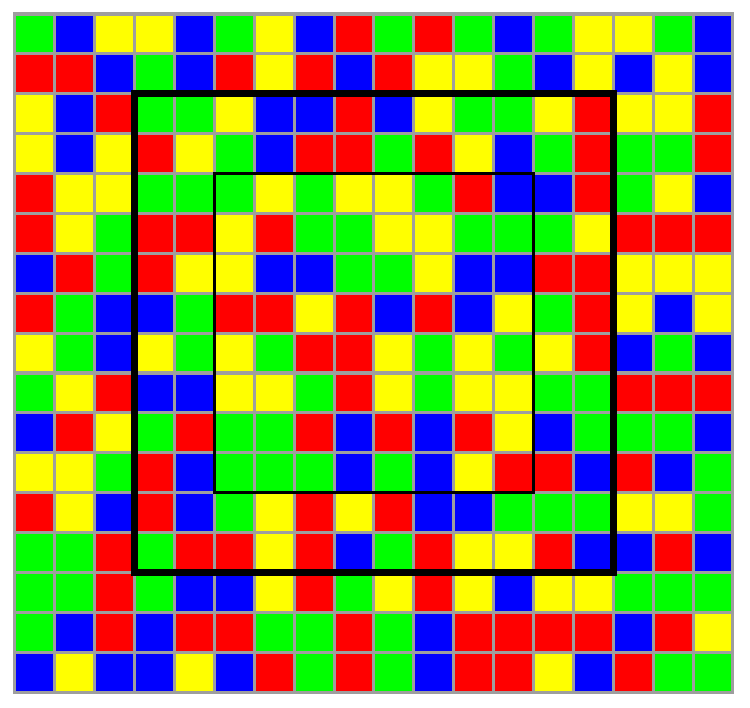
\includegraphics[width=0.45\textwidth]
{AKSs7colrBorderM1}\hspace{0.7cm}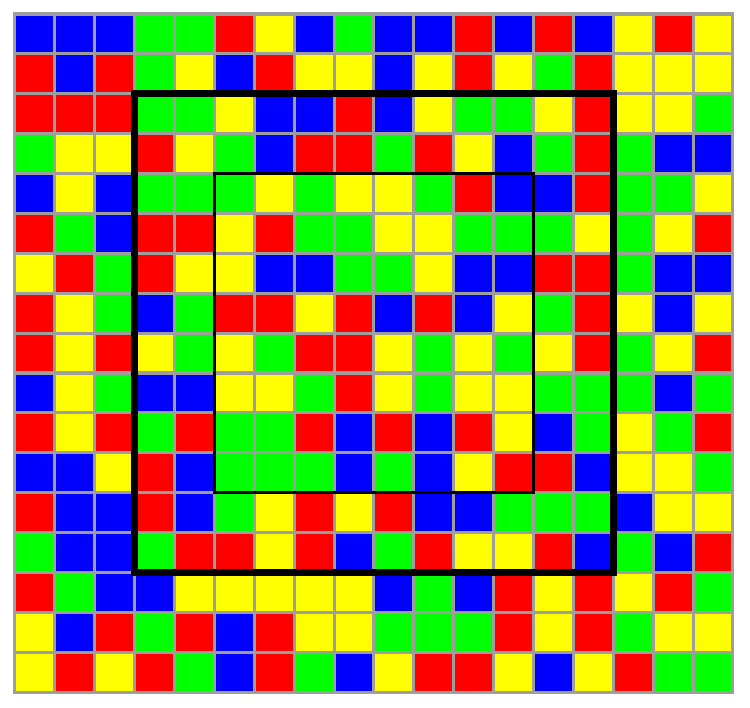
\includegraphics[width=0.45\textwidth]
{AKSs7colrBorderM2}
\end{center}
2d symbolic representation $\Mm_j$ of two {\twots} $\Xx_j$
shadowing each other within the shared
\brick\ $\Mm_{\R}$ %=\Mm_{\R_{0}} \cup \Mm_{\R_{1}}$ (blue)

\begin{itemize}
  \item border $\R$ (thick black) %, interior $\R_{0}$ (thin black)
  \item symbols outside \R\ differ
\end{itemize}
\vfill
$s=7/2$    \hfill                          Adrien Saremi 2017
%\label{fig:AKScloseActSymb}
%%%%%%%%%%%%%%%%%%%%%%%%%%%%%%%%%%%%%%%%%%%%%%%%%%%%%%%%%%%%%%%%%%%%%%%
\end{frame}

\begin{frame}{shadowing} %, \statesp}
%%%%%%%%%blogCats \label{fig:AKSs7dist} %%%%%%%%%%%%%%%%%%%%%%%%%%%%%
\begin{center}
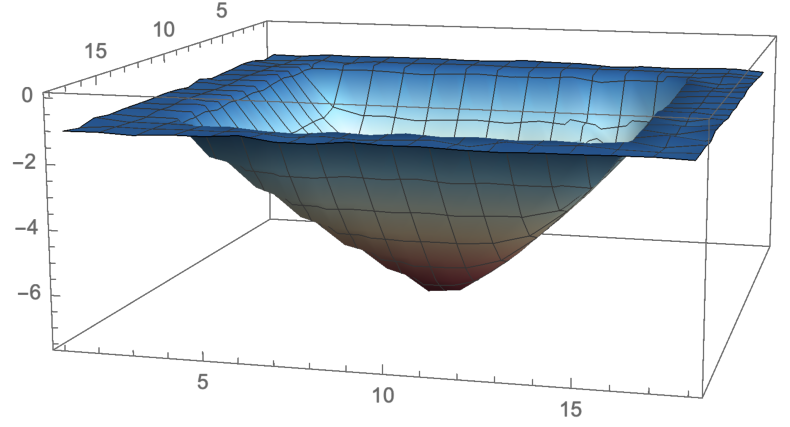
\includegraphics[width=0.65\textwidth]
{HL18ShadowingDistanceAverageLog3D}
\end{center}

\bigskip

the logarithm of the average of the absolute value of site-wise distance
\[
\ln|\ssp_{2,z}-\ssp_{1,z}|
\]
averaged over 250 solution pairs
\medskip

note the exponential falloff of the distance away from the center of the
shared \brick\ $\R$ %=\R_{0} \cup \R_{1}$.
\medskip

$\Rightarrow$ within the interior of the shared \brick,

\hfill \textcolor{blue}{shadowing is exponentially close}
\end{frame}

\begin{frame}{zeta function for a field theory ???} % much like Ising model}
% Ihara zeta functions ?
\begin{block}{`\po s' are now \twots\ (Bravais tiles)}
each a spacetime lattice tile  $p$ of area $A_p = L_p T_p$\\
that cover the \statesp\ with `natural weight'
\[
% Z(s) \approx
\sum_{p} \frac{e^{-A_p s}}
              {\left|\Det\jMorb_p\right|}
\]
\end{block}
%\begin{block}{symbolic dynamics : $d$\dmn}
%essential to encode shadowing
%\end{block}

\vfill
at this time :
\begin{itemize}
\item $d=1$ cat map zeta function works like charm
\item $d=2$ {\catlatt} works
\item $d\geq2$ Navier-Stokes  zeta is still but a dream
\end{itemize}
\end{frame}

\begin{frame}{}
\begin{enumerate}
              \item \textcolor{gray}{\small
%what this is about
%              \item
a coin toss
              \item
a kicked rotor
              \item
\catlatt
                  }
              \item {\Large
bye bye, dynamics
%                  }\textcolor{gray}{\small
%              \item
%bye bye, dynamics
                    }
            \end{enumerate}
\end{frame}

\section[bye bye, dynamics]
 {bye bye, dynamics}
\label{s:byeDynamics}

\begin{frame}{Bruno and Predrag in Kyoto, May 2006}
\begin{center}
\hfill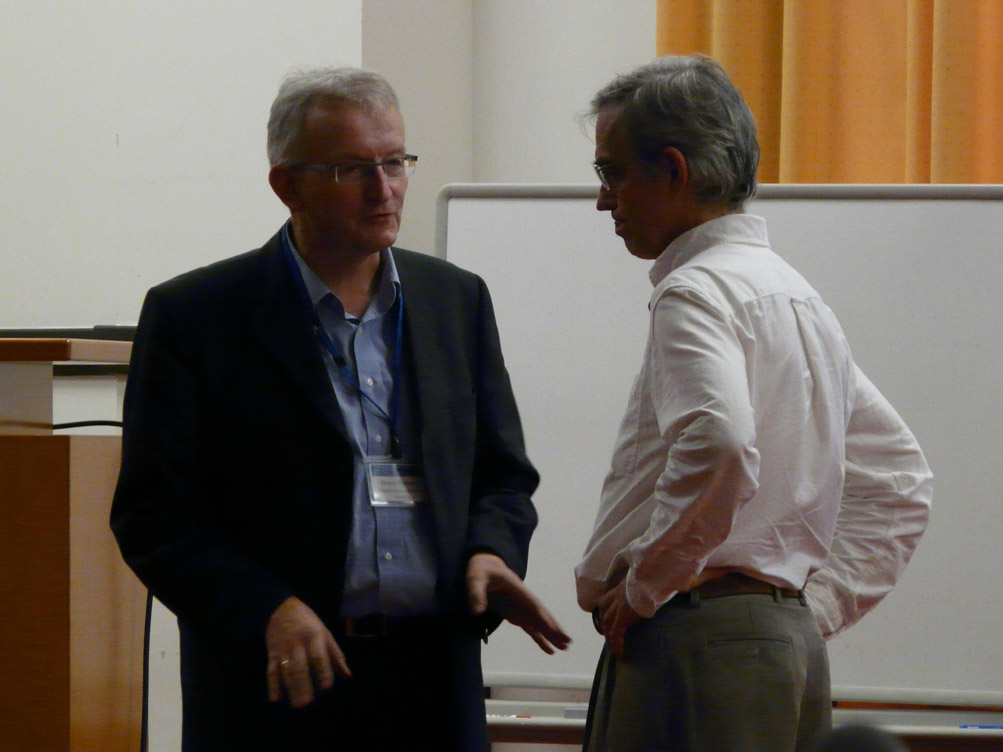
\includegraphics[width=1.00\textheight]{111130PC-EckhardtKyoto}
\end{center}
\end{frame}

\begin{frame}{insight 1 : how is turbulence described?}
\begin{block}{not by the evolution of an initial state}
exponentially unstable system have finite (Lyapunov) time and
space prediction horizons
\end{block}
but
\bigskip

\begin{block}{by enumeration of admissible field configurations}
and their natural weights
\end{block}
\end{frame}

\begin{frame}{insight 2 : symbolic dynamics for turbulent flows}
applies to
all PDEs with translational symmetries

\bigskip

a $d$\dmn\ spatiotemporal field configuration
\[
\{\ssp_{z}\} = \{\ssp_{z},  z\in \integers^{d}  \}
\]
is labelled by a \textcolor{red}{$d$\dmn} {spatiotemporal
{\brick}} of symbols
\[
\{\m_{z}\} = \{\m_{z}, z\in \integers^{d}\}
\,,
\]

\bigskip

rather than a \textcolor{red}{single} temporal symbol sequence

\bigskip

(as is done when describing a small coupled few-``body'' system, or a
small computational domain).
\end{frame}

\begin{frame}{insight 3 : description of turbulence by \twots}
\begin{block}{1 time, 0 space dimensions}
a {\statesp} point is {\em periodic} if its orbit returns to itself
after a finite time \period{}; such \textcolor{blue}{orbit tiles the time} axis
by infinitely many repeats
\end{block}

\bigskip

\begin{block}{1 time, $d$-1 space dimensions}
 a {\statesp} point is {\em spatiotemporally periodic} if
it belongs to \\ an invariant $d$-torus ${\R}$,\\
\ie, a \brick\ $\Mm_{\R}$ that
\textcolor{blue}{tiles the lattice state}  $\Mm$, \\
with period $\ell_j$ in $j$th lattice direction
\end{block}
\end{frame}

\begin{frame}{bye bye, dynamics}
\begin{enumerate}
              \item
challenge : describe states of turbulence in infinite spatiatemporal domains
              \item
theory : classify, enuremate all spatiotemporal tilings
              \item
example : \catlatt, the simplest model of ``turbulence''
\end{enumerate}

\vfill

there is no more time

\medskip

there is only enumeration of admissible spacetime field configurations
\end{frame}

\begin{frame}{in future there will be no future}
\begin{center}
{\huge goodbye}
\end{center}

\vfill

to long time and/or space integrators

\medskip

\hfill they never worked and could never work
\end{frame}

\begin{frame}{Mike, John, Predrag and Bruno, KITP - UCSB, February 2017}
\begin{center}
\hfill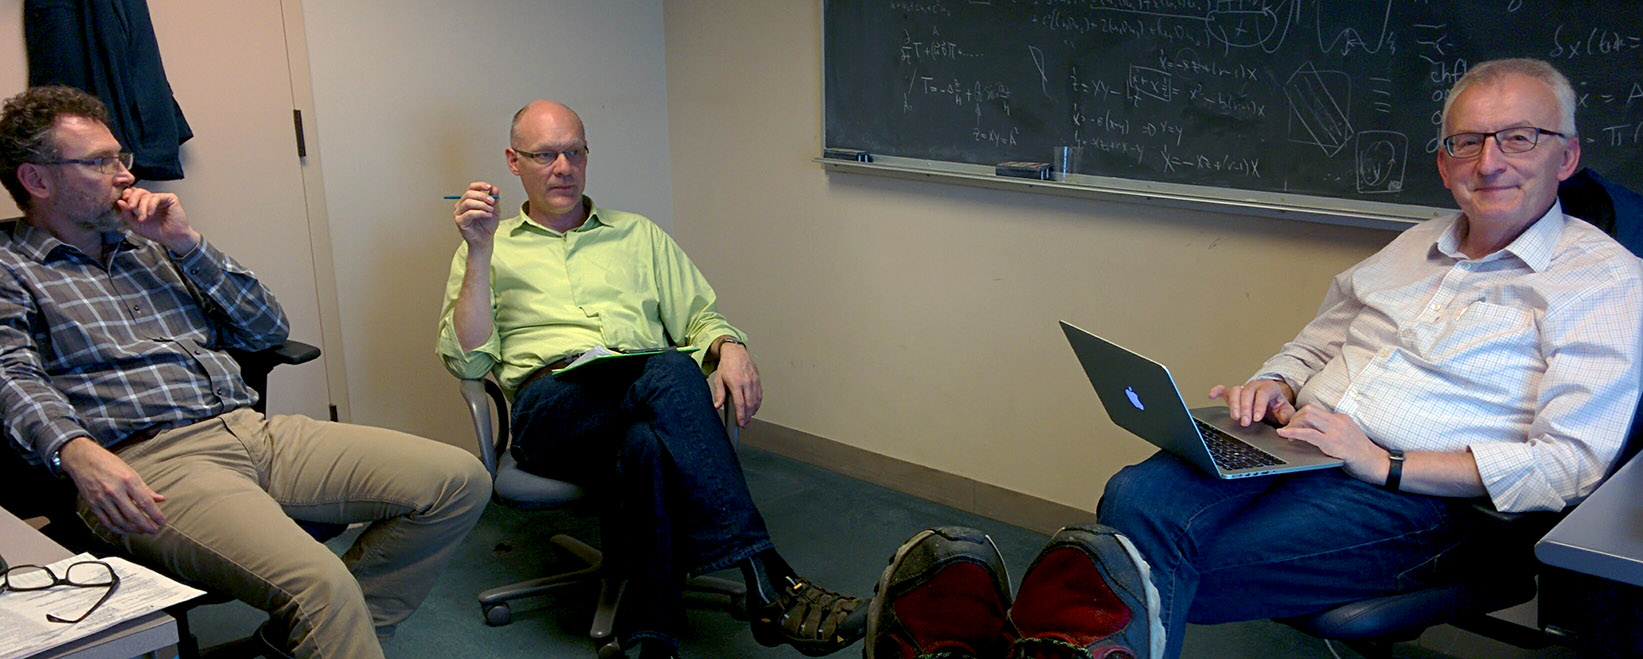
\includegraphics[width=1.00\textwidth]{20170208MikeJohnBruno}
\end{center}
\end{frame}

\end{document}
